\chapter{Concept}
\label{Concept}

This chapter covers the conceptual design of the navigation and defines requirements for some of its parts.\\

Based on the analysis in chapter \ref{relatedwork} the navigation stack seems to be a well fitting core structure for the navigation. The use case leads to modifications to the recommended setup, pictured in figure \ref{navigation stack setup}.

Afterwards the tasks of the nodes in move\_base need to be defined. These will be categorized into the global and local stage, each consisting of a planner and a costmap.
Additionally the setup requires nodes, which autonomously find new goals for the navigation and transform the sensor data into a usable format. 

\section{Sensor Transforms}
To know the position of every sensor relative to the robot and its odometry the tf\_tree has to be build. While this can be realized by calculating the transformations between the frames manually,  using the ROS package robot\_state\_publisher is a cleaner approach. This requires a robot description in URDF format that specifies the relations between everything mounted on the robot.\\

The required transform from the base to the odom frame is build by using the position derived from the wheel encoder data.

\section{Map}

The map is a representation of the robots environment. With it go and no-go zones can be determined.\\

Unfortunately, amcl and the map\_server are not suited for this use case, since they require a prerecorded map of the environment. 

A SLAM (simultaneous localization and mapping) algorithm becomes highly useful since the robot might drive multiple rounds, allowing it to build its own map.\\
This potentially allows a goal extraction from the map instead of estimating it by using the sensor data stream. Furthermore it can be used to determine the robots position relative to the map, by providing a transformation between the map and odom tf frames.

Unfortunately, the data that can be fed to the SLAM algorithm is very limited, since it is not guaranteed, that the lidar sensor all ways sees static obstacles. Another data source for the SLAM algorithm could be the points extracted from the road detection. Unfortunately, the road markings are similar to a corridor and do not have a lot of features, other than their curvature.\\

This significantly decreases the reliability of the map which therefore will highly depend on good odometry, since for example a straight section of the road always looks similar, even if it is on the other side of the circuit. The odometry provides an estimate, where the SLAM algorithm should attach the sensor data to the map.

To get a better map, both of the data inputs have to be used, which results in the need of a SLAM algorithm with multiple inputs.\\

\section{move\_base}

move\_base consist of a global and a local part, the combination of both defines the path finding characteristic of the navigation. Since each part has a different task they can be separated into the global and local stage.

\subsection{Global Stage}
The general task of the global planner is like described in the theoretical background to plan a rough path through the grid of the costmap, that does not collide with any lethal cell.\\

In this scenario the global planner will also be used to guide the robot on the correct lane. This results in the following requirements:

\begin{itemize}
	\item The global costmap needs information about the road markings and the obstacles detected by the lidar scan
	\item The global costmap needs to incorporate cost that generate a preference for the right lane, but allow the global path to go to the left lane in case of an obstacle
	\item The global planner has to respect all cost values
\end{itemize}

\subsection{Local Stage}
The local stage on the other hand has the task of finding a path, that is feasible for the dynamics of the robot and does not collide with objects.\\
This path is supposed to be close to the global path and follow its lane changes, but it needs to be able to separate itself from it, if necessary.

Therefore the local costmap needs to contain information about the road markings and the obstacles detected by the lidar scan.

\section{PoseFinder}
The job of this node is to extract a goal from the sensor data or the map.\\

The road detection is only able to detect the road to a certain distance. Everything beyond is unknown.\\
To allow the planners to generate smooth paths the distance, at which goals need to be found should be relatively far away from the robot. Therefore this node needs to estimate the upcoming course and repeatably send new goals. Since this approach uses estimations, it is uncertain if the goal is actually on the road or not.

If a map is available the estimation is redundant, since the map is likely to be more precise.

\section{Sensor Filter}

This block incorporates the nodes that process the sensor data into a format, that is usable for the navigation\_stack. 
Therefore it consists out of the following nodes:

\begin{itemize}
	\item \textbf{roadDetection} will extract approximated polynomials for the road markings and the lanes from the camera data
	\item \textbf{markfreespace} needs to publish point clouds to the costmaps and the SLAM algorithm consisting of the road detection data and the lidar scan.
\end{itemize}

Like described in the requirements, the simulator is supposed to produce realistic sensor data, which might need filtering. These filters are additionally located in this block.

\section{Resulting Concept}
The schematic in figure \ref{navconcept} shows the concept of the navigation.  To keep the schematic as simple as possible, not every connections between the nodes are highlighted (Appendix \ref{config} shows the finalized schematic).\\

\begin{figure}[H]
	\begin{center}
		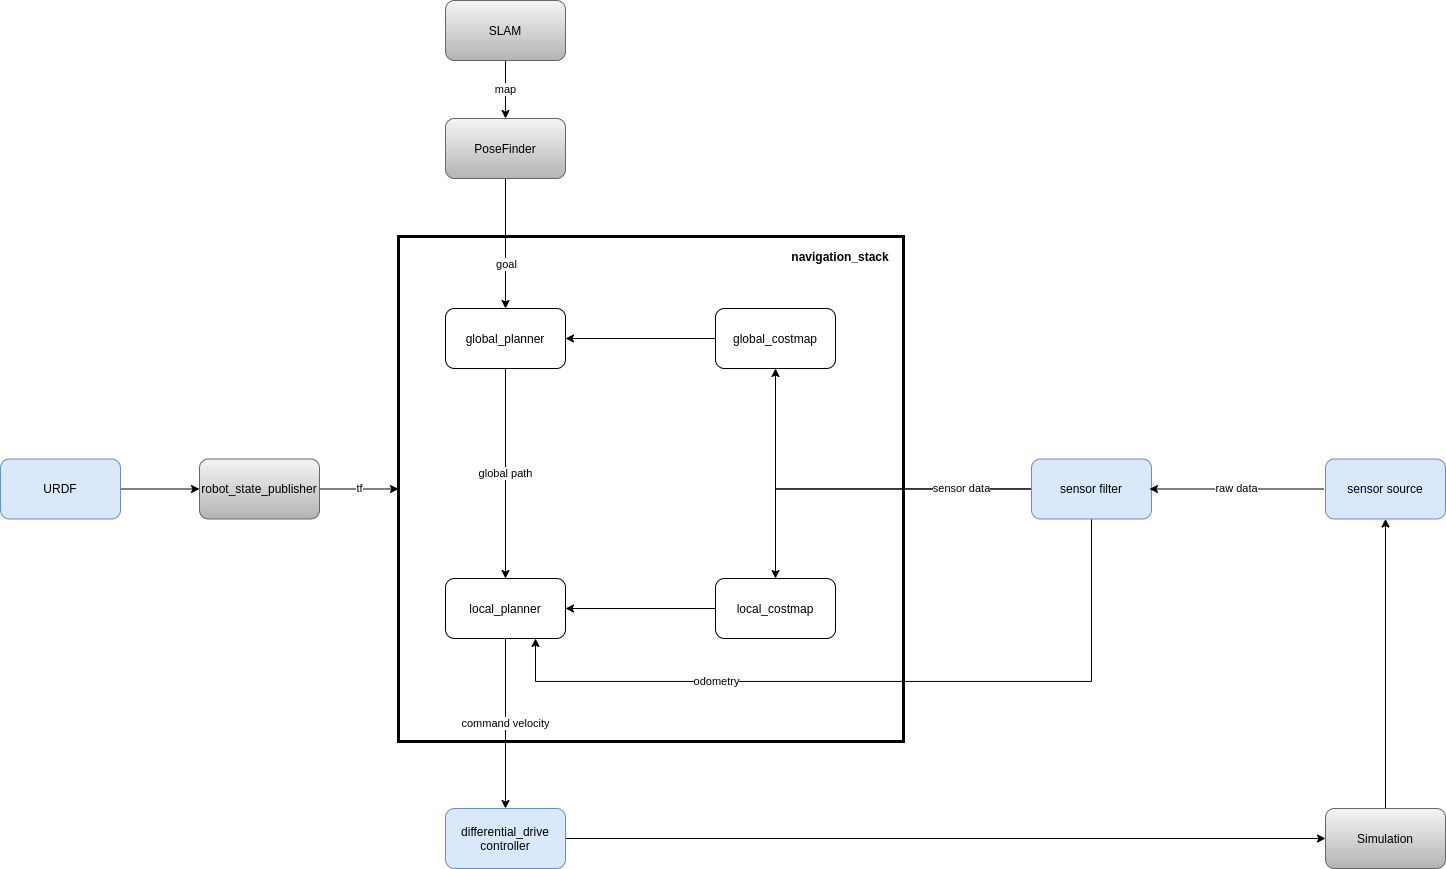
\includegraphics[width=140mm]{Pictures/Updated navigation concept}
		\caption[updated navigation concept]{Updated navigation concept (Blue - platform specific nodes, Grey - optional nodes, White - move\_base nodes)}
		\label{navconcept}
	\end{center}
\end{figure}



The PoseFinder will repeatedly find goals based on the current state of the map and the sensor data. The goals will then be handed over to the navigation stack. This uses the filtered sensor data to determine, where the robot is as well as, where it is allowed to go and where not. Afterwards the cascading planners produce first a rough, collision free, path on the correct lane and then a path that is possible for the dynamics of the robot. This path then gets converted to velocity commands and sent to the motor controller.\\




